\documentclass[a4paper]{article}

\usepackage[a4paper,margin=2cm]{geometry}
\usepackage[utf8]{inputenc}
\usepackage{times}
\usepackage[english]{babel}
\usepackage{multirow}
\usepackage{amsmath,graphicx}
\usepackage{hyperref}

\begin{document}

\begin{center}
  \Large Rudimant, the DFKI MLT dialogue engine
\end{center}

\section{Purpose}

The multimodal interaction manager analyses natural language coming from the
user, and generates natural language and gestures for the robot resp. its
virtual replacement, the avatar. The generation is based on incoming stimuli,
like speech or text input, or high-level action requests coming from some
strategic planning component, or any other sensor input, if available.

The goal is to create engaging interactions with the users that support the
currently active high-level goals.

\section{Interaction with the overall system}

The interaction manager will get several input types from the nexus, the ones
currently foreseen are: input from automatic speech recognition (ASR) or typed
natural input, user parameters, like name, age, hobbies, etc. but also more
dynamic ones like mood or health data, and also triggers from high-level
planning.

All these inputs are stored as RDF data, based on an ontology developed as part
of the interaction manager, and available to all other components as a data
format specification.

When new data is added, a set of declaratively specified reactive rules will
propose dialogue moves or other actions and send these proposals to the action
selection mechanism. The selection mechanism eventually selects one of the
proposed actions and sends it back. If the proposed action results in dialogue
acts, these are turned into verbal output and gestures with the help of a
multimodal generation component, which retrieves parameters from the RDF
database to adapt the generation to the user's likings, and can also take into
account sensory data such as her or his estimated mood.

\section{Internal structure}

As shown in the picture below, the interaction manager consists of the RDF
store, which also contains the functionality to store incoming data in the
format specified by the ontology, thereby making it readily accessible for
other components.

The second major component is the rule processor for the dialogue management
rules, which generates proposals for actions when new incoming data
arrives. The rules not only use the new data, but also the interaction history
stored in the RDF database to take its decisions.

The last two parts are a robust natural language interpretation module (not
explicitly shown in the picture), which turns spoken or written utterances
into dialogue acts, possibly with an intermediate step that involves a more
elaborate semantic format, and a multimodal generation component, which turns
outgoing dialogue acts into natural language utterances and gestures.

\vspace*{4ex}

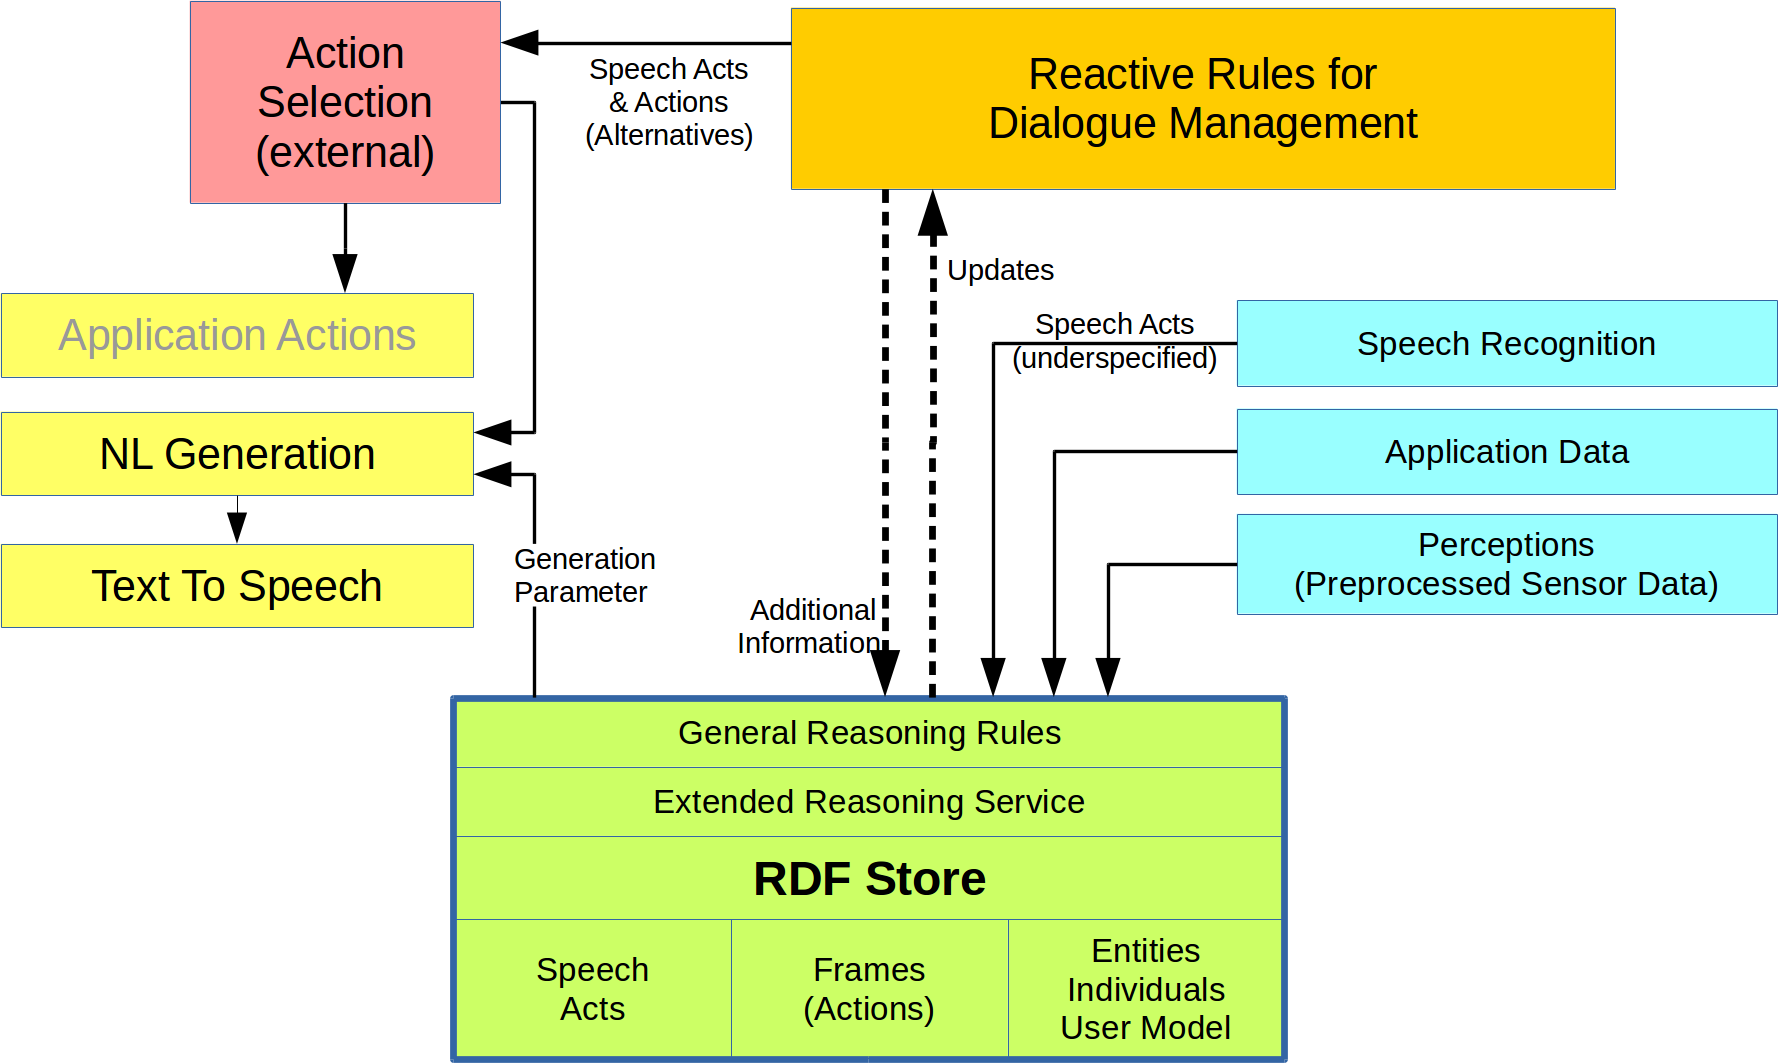
\includegraphics[width=.9\textwidth]{rudimant.png}

\section{Options for translating rules and .rudi files}

Naming convention: a label followed by a colon followed by an \emph{if} is
called \emph{rule} from now on.

There are two main options to translate:
\begin{itemize}
\item[A)] translate the whole project into one large Java class / method
  Problems with this approach
  \begin{itemize}
  \item The relation to the source code is hard to track: no modularity, one
    large blob
  \item The execution regime can not be changed except by changing the
    translation (no dynamic adaptation of execution)
  \end{itemize}
\item[B)] Create a class for each .rudi file and each top-level rule
  \begin{itemize}
  \item Clear structure that is isomorphic to the .rudi files
  \item Dynamic execution strategy is easier to imagine, albeit not really
    feasible (do we want/need it?)
  \item Variables on the top level of a file can be implemented by class
    fields and fully specified access, such as Introduction.special\_variable
  \end{itemize}
\end{itemize}

We're going for version B), assuming that most of the variables which have
non-local scope are state variables in the agent, which also might be
specified in special top-level files. These should also contain specifications
for general framework functions, i.e., the whole signatures including types
for the arguments and return types, to enable advanced type checking.

Similar files could be used for custom user state variables and functions,
i.e., for Quiz logic, custom knowledge bases, etc.

Embedded rules will be treated differently to avoid the overhead of handling
local scope and lifetime of variables.

\texttt{return} statements can have optional labels that indicate the exit
point / level, which may be local rule, top-level rule or file. A return
without label exits from the innermost scope.

Example for a top-level rule:

\begin{verbatim}
a:
if ( XXXX ) {
  x = child_27;
  b:
  if (YYYY) {
     x = child_3;
     c:
     if ( ZZZZ ) {
        ....
        if (....) return b:;
        ....
     } // c: ends
     ....
  } // b: ends
} // a: ends
\end{verbatim}

The labeled exits are implemented by setting flags in a bit mask that are
tested in the following to skip code not to be executed:
\newpage
Possible translation, (example starts at \texttt{return b:})
\begin{verbatim}
a:
if ( XXXX ) {
  x = child_27;
  b:
  if (YYYY) {
     x = child_3;
     c:
     if ( ZZZZ ) {
        ....
        if (....) {
           // return b:;
           returnMask |= b_mask;
        }
        if ((returnMask | (a_mask | b_mask | c_mask)) == 0) {
           ....
        }
     } // c: ends
     if ((returnMask | (a_mask | b_mask)) == 0) {
     ....
     }
  } // b: ends
  if ((returnMask | a_mask) == 0) {
  }
} // a: ends
\end{verbatim}

\section{Writing to Rudi (with care)}
If you are in a state where you want to immediately stop processing and leave all
rules, use a call to the method Agent.stopProcessing() to jump out of the topmost
rule file.

%%% Local Variables:
%%% mode: latex
%%% TeX-master: "master"
%%% End:


\end{document}
